% generated by Plantuml 1.2025.2       
\definecolor{plantucolor0000}{RGB}{255,255,255}
\definecolor{plantucolor0001}{RGB}{24,24,24}
\definecolor{plantucolor0002}{RGB}{0,0,0}
\definecolor{plantucolor0003}{RGB}{255,255,255}
\definecolor{plantucolor0004}{RGB}{226,226,240}
\definecolor{plantucolor0005}{RGB}{254,255,221}
\definecolor{plantucolor0006}{RGB}{238,238,238}
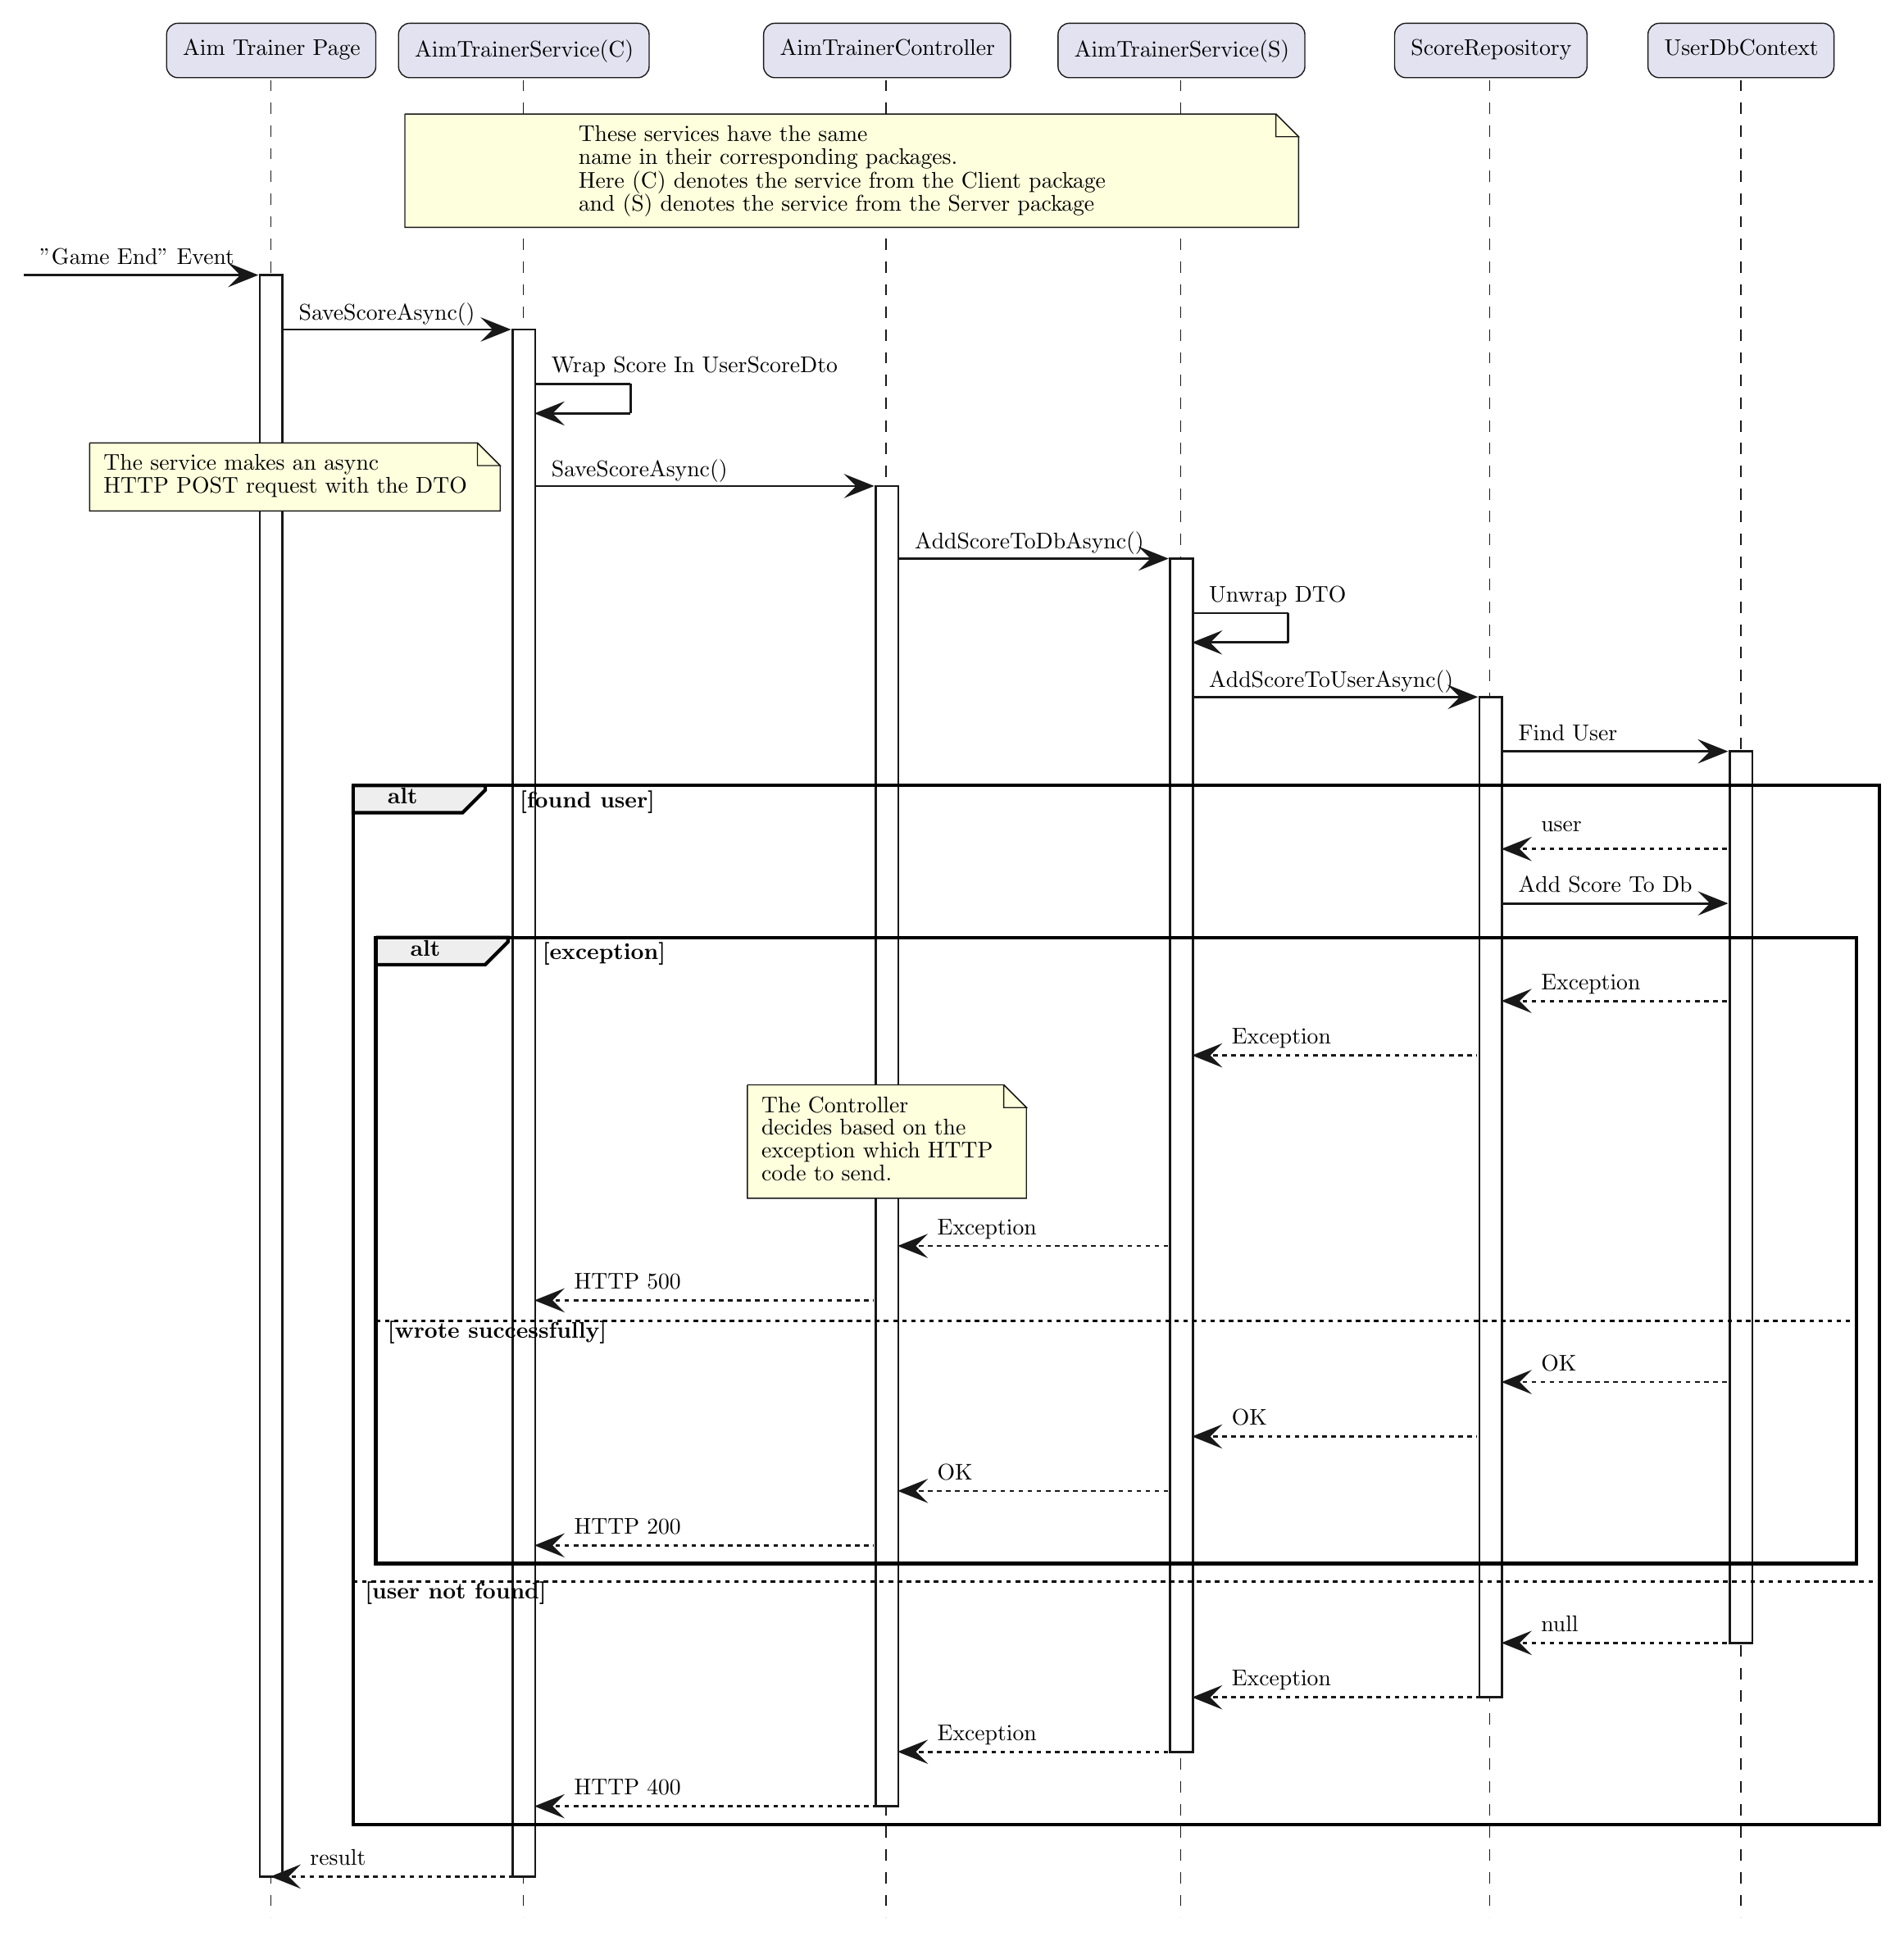
\begin{tikzpicture}[yscale=-1
,pstyle0/.style={color=plantucolor0001,fill=white,line width=1.0pt}
,pstyle1/.style={color=black,line width=1.5pt}
,pstyle2/.style={color=plantucolor0003,line width=0.0pt}
,pstyle3/.style={color=plantucolor0001,line width=0.5pt,dash pattern=on 5.0pt off 5.0pt}
,pstyle4/.style={color=plantucolor0001,fill=plantucolor0004,line width=0.5pt}
,pstyle5/.style={color=plantucolor0001,fill=plantucolor0005,line width=0.5pt}
,pstyle6/.style={color=plantucolor0001,fill=plantucolor0001,line width=1.0pt}
,pstyle7/.style={color=plantucolor0001,line width=1.0pt}
,pstyle8/.style={color=black,fill=plantucolor0006,line width=1.5pt}
,pstyle9/.style={color=plantucolor0001,line width=1.0pt,dash pattern=on 2.0pt off 2.0pt}
,pstyle10/.style={color=black,line width=1.0pt,dash pattern=on 2.0pt off 2.0pt}
]
\draw[pstyle0] (104.07pt,116pt) rectangle (114.07pt,822pt);
\draw[pstyle0] (215.435pt,140pt) rectangle (225.435pt,822pt);
\draw[pstyle0] (375.575pt,209pt) rectangle (385.575pt,791pt);
\draw[pstyle0] (505.365pt,241pt) rectangle (515.365pt,767pt);
\draw[pstyle0] (641.755pt,302pt) rectangle (651.755pt,743pt);
\draw[pstyle0] (752.035pt,326pt) rectangle (762.035pt,719pt);
\draw[pstyle1] (145.195pt,341pt) rectangle (818.035pt,799pt);
\draw[pstyle1] (155.195pt,408pt) rectangle (808.035pt,684pt);
\draw[pstyle2] (105.07pt,30pt) rectangle (113.07pt,840pt);
\draw[pstyle3] (108.945pt,30pt) -- (108.945pt,840pt);
\draw[pstyle2] (216.435pt,30pt) rectangle (224.435pt,840pt);
\draw[pstyle3] (220.195pt,30pt) -- (220.195pt,840pt);
\draw[pstyle2] (376.575pt,30pt) rectangle (384.575pt,840pt);
\draw[pstyle3] (380.15pt,30pt) -- (380.15pt,840pt);
\draw[pstyle2] (506.365pt,30pt) rectangle (514.365pt,840pt);
\draw[pstyle3] (509.955pt,30pt) -- (509.955pt,840pt);
\draw[pstyle2] (642.755pt,30pt) rectangle (650.755pt,840pt);
\draw[pstyle3] (646.35pt,30pt) -- (646.35pt,840pt);
\draw[pstyle2] (753.035pt,30pt) rectangle (761.035pt,840pt);
\draw[pstyle3] (757.035pt,30pt) -- (757.035pt,840pt);
\draw[pstyle4] (62.945pt,10pt) arc (180:270:5pt) -- (67.945pt,5pt) -- (150.195pt,5pt) arc (270:360:5pt) -- (155.195pt,10pt) -- (155.195pt,24pt) arc (0:90:5pt) -- (150.195pt,29pt) -- (67.945pt,29pt) arc (90:180:5pt) -- (62.945pt,24pt) -- cycle;
\node at (69.945pt,12pt)[below right,color=black,inner sep=0]{Aim Trainer Page};
\draw[pstyle4] (165.195pt,10pt) arc (180:270:5pt) -- (170.195pt,5pt) -- (270.675pt,5pt) arc (270:360:5pt) -- (275.675pt,10pt) -- (275.675pt,24pt) arc (0:90:5pt) -- (270.675pt,29pt) -- (170.195pt,29pt) arc (90:180:5pt) -- (165.195pt,24pt) -- cycle;
\node at (172.195pt,12pt)[below right,color=black,inner sep=0]{AimTrainerService(C)};
\draw[pstyle4] (326.15pt,10pt) arc (180:270:5pt) -- (331.15pt,5pt) -- (430pt,5pt) arc (270:360:5pt) -- (435pt,10pt) -- (435pt,24pt) arc (0:90:5pt) -- (430pt,29pt) -- (331.15pt,29pt) arc (90:180:5pt) -- (326.15pt,24pt) -- cycle;
\node at (333.15pt,12pt)[below right,color=black,inner sep=0]{AimTrainerController};
\draw[pstyle4] (455.955pt,10pt) arc (180:270:5pt) -- (460.955pt,5pt) -- (559.775pt,5pt) arc (270:360:5pt) -- (564.775pt,10pt) -- (564.775pt,24pt) arc (0:90:5pt) -- (559.775pt,29pt) -- (460.955pt,29pt) arc (90:180:5pt) -- (455.955pt,24pt) -- cycle;
\node at (462.955pt,12pt)[below right,color=black,inner sep=0]{AimTrainerService(S)};
\draw[pstyle4] (604.35pt,10pt) arc (180:270:5pt) -- (609.35pt,5pt) -- (684.16pt,5pt) arc (270:360:5pt) -- (689.16pt,10pt) -- (689.16pt,24pt) arc (0:90:5pt) -- (684.16pt,29pt) -- (609.35pt,29pt) arc (90:180:5pt) -- (604.35pt,24pt) -- cycle;
\node at (611.35pt,12pt)[below right,color=black,inner sep=0]{ScoreRepository};
\draw[pstyle4] (716.035pt,10pt) arc (180:270:5pt) -- (721.035pt,5pt) -- (793.035pt,5pt) arc (270:360:5pt) -- (798.035pt,10pt) -- (798.035pt,24pt) arc (0:90:5pt) -- (793.035pt,29pt) -- (721.035pt,29pt) arc (90:180:5pt) -- (716.035pt,24pt) -- cycle;
\node at (723.035pt,12pt)[below right,color=black,inner sep=0]{UserDbContext};
\draw[pstyle0] (104.07pt,116pt) rectangle (114.07pt,822pt);
\draw[pstyle0] (215.435pt,140pt) rectangle (225.435pt,822pt);
\draw[pstyle0] (375.575pt,209pt) rectangle (385.575pt,791pt);
\draw[pstyle0] (505.365pt,241pt) rectangle (515.365pt,767pt);
\draw[pstyle0] (641.755pt,302pt) rectangle (651.755pt,743pt);
\draw[pstyle0] (752.035pt,326pt) rectangle (762.035pt,719pt);
\draw[pstyle5] (168pt,45pt) -- (168pt,95pt) -- (562pt,95pt) -- (562pt,55pt) -- (552pt,45pt) -- (168pt,45pt);
\draw[pstyle5] (552pt,45pt) -- (552pt,55pt) -- (562pt,55pt) -- (552pt,45pt);
\node at (244.325pt,50pt)[below right,color=black,inner sep=0]{These services have the same};
\node at (244.325pt,60pt)[below right,color=black,inner sep=0]{name in their corresponding packages.};
\node at (244.325pt,70pt)[below right,color=black,inner sep=0]{Here (C) denotes the service from the Client package};
\node at (244.325pt,80pt)[below right,color=black,inner sep=0]{and (S) denotes the service from the Server package};
\draw[pstyle6] (92.07pt,112pt) -- (102.07pt,116pt) -- (92.07pt,120pt) -- (96.07pt,116pt) -- cycle;
\draw[pstyle7] (0pt,116pt) -- (98.07pt,116pt);
\node at (7pt,104pt)[below right,color=black,inner sep=0]{"Game End" Event};
\draw[pstyle6] (203.435pt,136pt) -- (213.435pt,140pt) -- (203.435pt,144pt) -- (207.435pt,140pt) -- cycle;
\draw[pstyle7] (114.07pt,140pt) -- (209.435pt,140pt);
\node at (121.07pt,128pt)[below right,color=black,inner sep=0]{SaveScoreAsync()};
\draw[pstyle7] (225.435pt,164pt) -- (267.435pt,164pt);
\draw[pstyle7] (267.435pt,164pt) -- (267.435pt,177pt);
\draw[pstyle7] (226.435pt,177pt) -- (267.435pt,177pt);
\draw[pstyle6] (236.435pt,173pt) -- (226.435pt,177pt) -- (236.435pt,181pt) -- (232.435pt,177pt) -- cycle;
\node at (232.435pt,152pt)[below right,color=black,inner sep=0]{Wrap Score In UserScoreDto};
\draw[pstyle6] (363.575pt,205pt) -- (373.575pt,209pt) -- (363.575pt,213pt) -- (367.575pt,209pt) -- cycle;
\draw[pstyle7] (225.435pt,209pt) -- (369.575pt,209pt);
\node at (232.435pt,197pt)[below right,color=black,inner sep=0]{SaveScoreAsync()};
\draw[pstyle5] (29pt,190pt) -- (29pt,220pt) -- (210pt,220pt) -- (210pt,200pt) -- (200pt,190pt) -- (29pt,190pt);
\draw[pstyle5] (200pt,190pt) -- (200pt,200pt) -- (210pt,200pt) -- (200pt,190pt);
\node at (35pt,195pt)[below right,color=black,inner sep=0]{The service makes an async};
\node at (35pt,205pt)[below right,color=black,inner sep=0]{HTTP POST request with the DTO};
\draw[pstyle6] (493.365pt,237pt) -- (503.365pt,241pt) -- (493.365pt,245pt) -- (497.365pt,241pt) -- cycle;
\draw[pstyle7] (385.575pt,241pt) -- (499.365pt,241pt);
\node at (392.575pt,229pt)[below right,color=black,inner sep=0]{AddScoreToDbAsync()};
\draw[pstyle7] (515.365pt,265pt) -- (557.365pt,265pt);
\draw[pstyle7] (557.365pt,265pt) -- (557.365pt,278pt);
\draw[pstyle7] (516.365pt,278pt) -- (557.365pt,278pt);
\draw[pstyle6] (526.365pt,274pt) -- (516.365pt,278pt) -- (526.365pt,282pt) -- (522.365pt,278pt) -- cycle;
\node at (522.365pt,253pt)[below right,color=black,inner sep=0]{Unwrap DTO};
\draw[pstyle6] (629.755pt,298pt) -- (639.755pt,302pt) -- (629.755pt,306pt) -- (633.755pt,302pt) -- cycle;
\draw[pstyle7] (515.365pt,302pt) -- (635.755pt,302pt);
\node at (522.365pt,290pt)[below right,color=black,inner sep=0]{AddScoreToUserAsync()};
\draw[pstyle6] (740.035pt,322pt) -- (750.035pt,326pt) -- (740.035pt,330pt) -- (744.035pt,326pt) -- cycle;
\draw[pstyle7] (651.755pt,326pt) -- (746.035pt,326pt);
\node at (658.755pt,314pt)[below right,color=black,inner sep=0]{Find User};
\draw[pstyle8] (145.195pt,341pt) -- (203.445pt,341pt) -- (203.445pt,343pt) -- (193.445pt,353pt) -- (145.195pt,353pt) -- (145.195pt,341pt);
\draw[pstyle1] (145.195pt,341pt) rectangle (818.035pt,799pt);
\node at (160.195pt,342pt)[below right,color=black,inner sep=0]{\textbf{alt}};
\node at (218.445pt,343pt)[below right,color=black,inner sep=0]{\textbf{[found user]}};
\draw[pstyle6] (662.755pt,365pt) -- (652.755pt,369pt) -- (662.755pt,373pt) -- (658.755pt,369pt) -- cycle;
\draw[pstyle9] (656.755pt,369pt) -- (751.035pt,369pt);
\node at (668.755pt,357pt)[below right,color=black,inner sep=0]{user};
\draw[pstyle6] (740.035pt,389pt) -- (750.035pt,393pt) -- (740.035pt,397pt) -- (744.035pt,393pt) -- cycle;
\draw[pstyle7] (651.755pt,393pt) -- (746.035pt,393pt);
\node at (658.755pt,381pt)[below right,color=black,inner sep=0]{Add Score To Db};
\draw[pstyle8] (155.195pt,408pt) -- (213.445pt,408pt) -- (213.445pt,410pt) -- (203.445pt,420pt) -- (155.195pt,420pt) -- (155.195pt,408pt);
\draw[pstyle1] (155.195pt,408pt) rectangle (808.035pt,684pt);
\node at (170.195pt,409pt)[below right,color=black,inner sep=0]{\textbf{alt}};
\node at (228.445pt,410pt)[below right,color=black,inner sep=0]{\textbf{[exception]}};
\draw[pstyle6] (662.755pt,432pt) -- (652.755pt,436pt) -- (662.755pt,440pt) -- (658.755pt,436pt) -- cycle;
\draw[pstyle9] (656.755pt,436pt) -- (751.035pt,436pt);
\node at (668.755pt,424pt)[below right,color=black,inner sep=0]{Exception};
\draw[pstyle6] (526.365pt,456pt) -- (516.365pt,460pt) -- (526.365pt,464pt) -- (522.365pt,460pt) -- cycle;
\draw[pstyle9] (520.365pt,460pt) -- (640.755pt,460pt);
\node at (532.365pt,448pt)[below right,color=black,inner sep=0]{Exception};
\draw[pstyle5] (319pt,473pt) -- (319pt,523pt) -- (442pt,523pt) -- (442pt,483pt) -- (432pt,473pt) -- (319pt,473pt);
\draw[pstyle5] (432pt,473pt) -- (432pt,483pt) -- (442pt,483pt) -- (432pt,473pt);
\node at (325pt,478pt)[below right,color=black,inner sep=0]{The Controller};
\node at (325pt,488pt)[below right,color=black,inner sep=0]{decides based on the};
\node at (325pt,498pt)[below right,color=black,inner sep=0]{exception which HTTP};
\node at (325pt,508pt)[below right,color=black,inner sep=0]{code to send.};
\draw[pstyle6] (396.575pt,540pt) -- (386.575pt,544pt) -- (396.575pt,548pt) -- (392.575pt,544pt) -- cycle;
\draw[pstyle9] (390.575pt,544pt) -- (504.365pt,544pt);
\node at (402.575pt,532pt)[below right,color=black,inner sep=0]{Exception};
\draw[pstyle6] (236.435pt,564pt) -- (226.435pt,568pt) -- (236.435pt,572pt) -- (232.435pt,568pt) -- cycle;
\draw[pstyle9] (230.435pt,568pt) -- (374.575pt,568pt);
\node at (242.435pt,556pt)[below right,color=black,inner sep=0]{HTTP 500};
\draw[pstyle10] (155.195pt,577pt) -- (808.035pt,577pt);
\node at (160.195pt,577pt)[below right,color=black,inner sep=0]{\textbf{[wrote successfully]}};
\draw[pstyle6] (662.755pt,600pt) -- (652.755pt,604pt) -- (662.755pt,608pt) -- (658.755pt,604pt) -- cycle;
\draw[pstyle9] (656.755pt,604pt) -- (751.035pt,604pt);
\node at (668.755pt,592pt)[below right,color=black,inner sep=0]{OK};
\draw[pstyle6] (526.365pt,624pt) -- (516.365pt,628pt) -- (526.365pt,632pt) -- (522.365pt,628pt) -- cycle;
\draw[pstyle9] (520.365pt,628pt) -- (640.755pt,628pt);
\node at (532.365pt,616pt)[below right,color=black,inner sep=0]{OK};
\draw[pstyle6] (396.575pt,648pt) -- (386.575pt,652pt) -- (396.575pt,656pt) -- (392.575pt,652pt) -- cycle;
\draw[pstyle9] (390.575pt,652pt) -- (504.365pt,652pt);
\node at (402.575pt,640pt)[below right,color=black,inner sep=0]{OK};
\draw[pstyle6] (236.435pt,672pt) -- (226.435pt,676pt) -- (236.435pt,680pt) -- (232.435pt,676pt) -- cycle;
\draw[pstyle9] (230.435pt,676pt) -- (374.575pt,676pt);
\node at (242.435pt,664pt)[below right,color=black,inner sep=0]{HTTP 200};
\draw[pstyle10] (145.195pt,692pt) -- (818.035pt,692pt);
\node at (150.195pt,692pt)[below right,color=black,inner sep=0]{\textbf{[user not found]}};
\draw[pstyle6] (662.755pt,715pt) -- (652.755pt,719pt) -- (662.755pt,723pt) -- (658.755pt,719pt) -- cycle;
\draw[pstyle9] (656.755pt,719pt) -- (756.035pt,719pt);
\node at (668.755pt,707pt)[below right,color=black,inner sep=0]{null};
\draw[pstyle6] (526.365pt,739pt) -- (516.365pt,743pt) -- (526.365pt,747pt) -- (522.365pt,743pt) -- cycle;
\draw[pstyle9] (520.365pt,743pt) -- (645.755pt,743pt);
\node at (532.365pt,731pt)[below right,color=black,inner sep=0]{Exception};
\draw[pstyle6] (396.575pt,763pt) -- (386.575pt,767pt) -- (396.575pt,771pt) -- (392.575pt,767pt) -- cycle;
\draw[pstyle9] (390.575pt,767pt) -- (509.365pt,767pt);
\node at (402.575pt,755pt)[below right,color=black,inner sep=0]{Exception};
\draw[pstyle6] (236.435pt,787pt) -- (226.435pt,791pt) -- (236.435pt,795pt) -- (232.435pt,791pt) -- cycle;
\draw[pstyle9] (230.435pt,791pt) -- (379.575pt,791pt);
\node at (242.435pt,779pt)[below right,color=black,inner sep=0]{HTTP 400};
\draw[pstyle6] (120.07pt,818pt) -- (110.07pt,822pt) -- (120.07pt,826pt) -- (116.07pt,822pt) -- cycle;
\draw[pstyle9] (114.07pt,822pt) -- (219.435pt,822pt);
\node at (126.07pt,810pt)[below right,color=black,inner sep=0]{result};
\end{tikzpicture}
